\label{appendix:helicene}
Some experiments were done to test the thermal stability of the self-assembly. Therefor the molecules are deposited at room temperature in subsequently annealed to higher temperatures and investigated in LT-STM (\autoref{fig:hel-fig-S1}). Moderate annealing to \SI{100}{\celsius} leads to almost no changes, the chains maintain their shapes. At intermediate temperatures a ring closure reaction between the first and last carbon ring is induced, resulting in a new species. Its appearance is flat in LT-STM. As the temperature increases, they start to disintegrate into smaller fragments with no dominant binding motif.

\begin{figure} \centering
	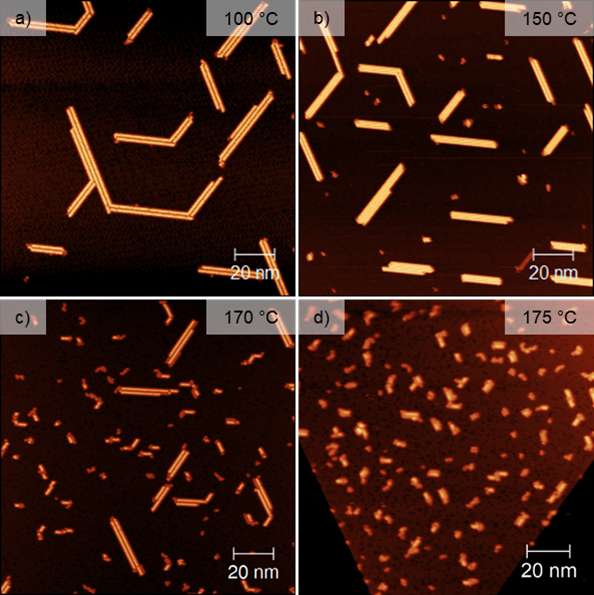
\includegraphics[width=0.7\textwidth]{./images/paper/helicene/fig-S1}
	\caption{After adsorption at RT on Ag(111) the same sample was subsequently heated to 100/150/170 \SI{}{\celsius} (a-c) and investigated in LT-STM. The higher the annealing temperature gets, the shorter the chains become. At intermediate temperature ring closure reactions form flat compounds. At longer annealing times at elevated temperature (\SI{175}{\celsius}, \SI{30}{\minute}, d) the molecules start to form denser but more unordered configurations while the typical chain length of the assembly further decreases.}
	\label{fig:hel-fig-S1}
\end{figure}

A closer look revealed that some of the molecules start to change their appearance after annealing.  The height of single molecules reduces and the distinct bright spot in the molecule vanishes (\autoref{fig:hel-fig-S1}a)). Modelling a dcdb-[5]H with Hyperchem (AM1) where first and last carbon rings are fused together matches this shape very well, pointing to an temperature induced ring closure reaction (\autoref{fig:hel-fig-S2}b)), which suppresses chirality of the new formed species. These often but not attach to the initial molecular assembly or agglomerate in unordered configurations. A cyclodehydogenation is observed for double 5[H] on Au(111) at \SI{380}{\celsius} \cite{Wang_Heteroatom-doped_2017} and dibenzo[i,o]heptahelicene on Ag(111) at \SIrange{247}{397}{\celsius} \cite{Stetsovych_helical_2016}. Heptahelicene/Cu(111) decomposes above \SI{227}{\celsius} \cite{Ernst_two-dimensional_2001}. Investigation of [7]H on Ni(111) and Ni(100) revealed dehydrogenation temperatures not below \SI{227}{\celsius} and \SI{127}{\celsius} respectively.\cite{Ernst_Adsorption_2003}

\begin{figure} \centering
	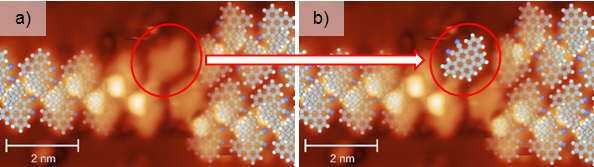
\includegraphics[width=0.7\textwidth]{./images/paper/helicene/fig-S2}
	\caption{Upon heating to the Ag(111) to \SI{170}{\celsius} for \SI{10}{\minute} some molecules start to change their typical appearance (red circle in a)). They lose their bright feature and become flat. A molecule’s model representation with its first and last carbon rings connected is shown in b) closely resembling the footprint of the new species.}
	\label{fig:hel-fig-S2}
\end{figure}

Chains formed at RT on Ag(111) bear significantly more molecules than those formed on Ag(100) and are almost exclusively made of two strands - thus are 4 molecules wide. This is shown as histogram representation in \autoref{fig:hel-fig-S4}. Only some chains are three strands wide.

\begin{figure} \centering
	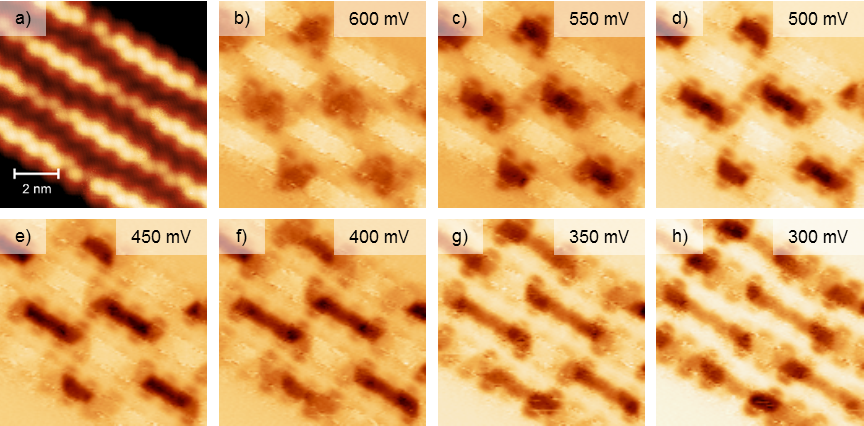
\includegraphics[width=0.7\textwidth]{./images/paper/helicene/fig-S3}
	\caption{(a) Topography of a molecular chain along the Ag(100) high symmetry direction recorded at \SI{400}{\milli \volt}. (b-h) dI/dV  maps ranging from \SIrange{600}{300}{\milli \volt}. The periodic height modulation visible in the topography can be recognized in the dI/dV maps. The width of the features decreases with decreasing bias voltage.}
	\label{fig:hel-fig-S3}
\end{figure}

\begin{figure} \centering
	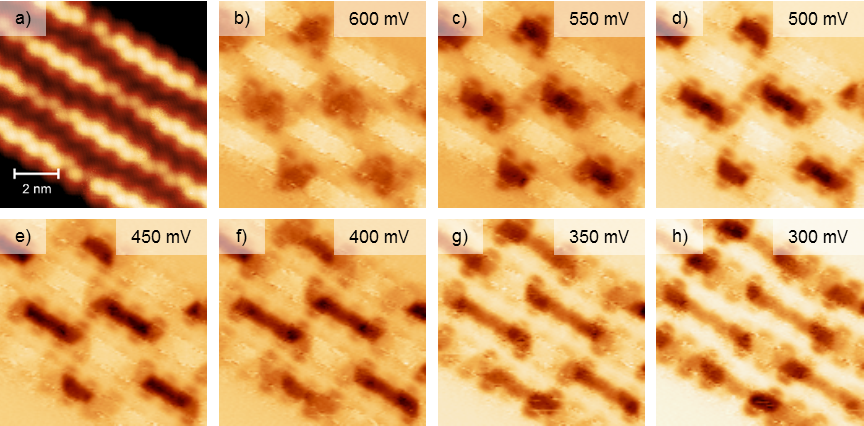
\includegraphics[width=0.7\textwidth]{./images/paper/helicene/fig-S3}
	\caption{Chain length (a) and width (b) of dcdb-5[H] assemblies after RT adsorption on Ag(111). Chains are made up strands with each strand being two molecules wide - resulting in an even chain width.}
	\label{fig:hel-fig-S4}
\end{figure}
